% Befehl \fibelvorstellung: Erstellt die Vorstellung eines FSlers mit Bild
%	Parameter #1: Bild (wrapfigure)
%	Parameter #2: Text
\newcommand{\fibelvorstellung}[2]{%
	\begin{minipage}{\columnwidth}
		% Kein Abstand vor bzw. nach Bildern bei wrapfigure
		\setlength{\intextsep}{0cm}
		% geringfügiger Abstand zwischen Paragraphen
		\setlength{\parskip}{0.5ex}
		#1
		#2
		\vspace{0.5ex}
	\end{minipage}
	
	\vspace{5ex plus 2ex minus 1ex}
}
\newlength{\fibelstdlen}
\setlength{\fibelstdlen}{3.7cm}

\section{Der Fachschaftsrat~(FSR) Physik stellt sich vor}
\begin{multicols}{2}
\small


\fibelvorstellung{
	\begin{wrapfigure}{l}{0cm}
		\includegraphics[width=\fibelstdlen]{res/vorstellungsfotos/michael_te_vrugt}
	\end{wrapfigure}
}
{
Hi, ich bin Michael und promoviere gerade in Physik und Philosophie. In der Fachschaft bin ich seit Jahren aktiv und momentan u.A. für die Master-Infoveranstaltung zuständig. 
Bei Fragen zu Philosophie, einem Auslandsjahr, Doppelstudium oder Stipendium - und natürlich auch allem anderen - seid ihr bei mir genau richtig. 
Ansonsten wünsche ich euch viel Spaß in der O-Woche, und vielleicht sieht man sich mal bei einer Fachschaftssitzung. :)
}

\vspace{-0.8cm}

\fibelvorstellung{
	\begin{wrapfigure}{r}{0cm}
		\includegraphics[width=\fibelstdlen]{res/vorstellungsfotos/kristin_nissen.jpg}
	\end{wrapfigure}
}
{
Hey ihr lieben! Ich bin Kristin und nun im 1. Semester meines Physikmasters. Ich kümmere mich in der Fachschaft um die Evaluation und auch um die Homepage. 
Falls ihr irgendwelche Fragen habt werde ich euch liebend gerne weiter helfen. Nun wünsche ich euch erstmal einen reibungsfreien Studienbeginn und viel Spaß in Münster. 
}

\vspace{-0.6cm}

\fibelvorstellung{
	\begin{wrapfigure}{l}{0cm}
		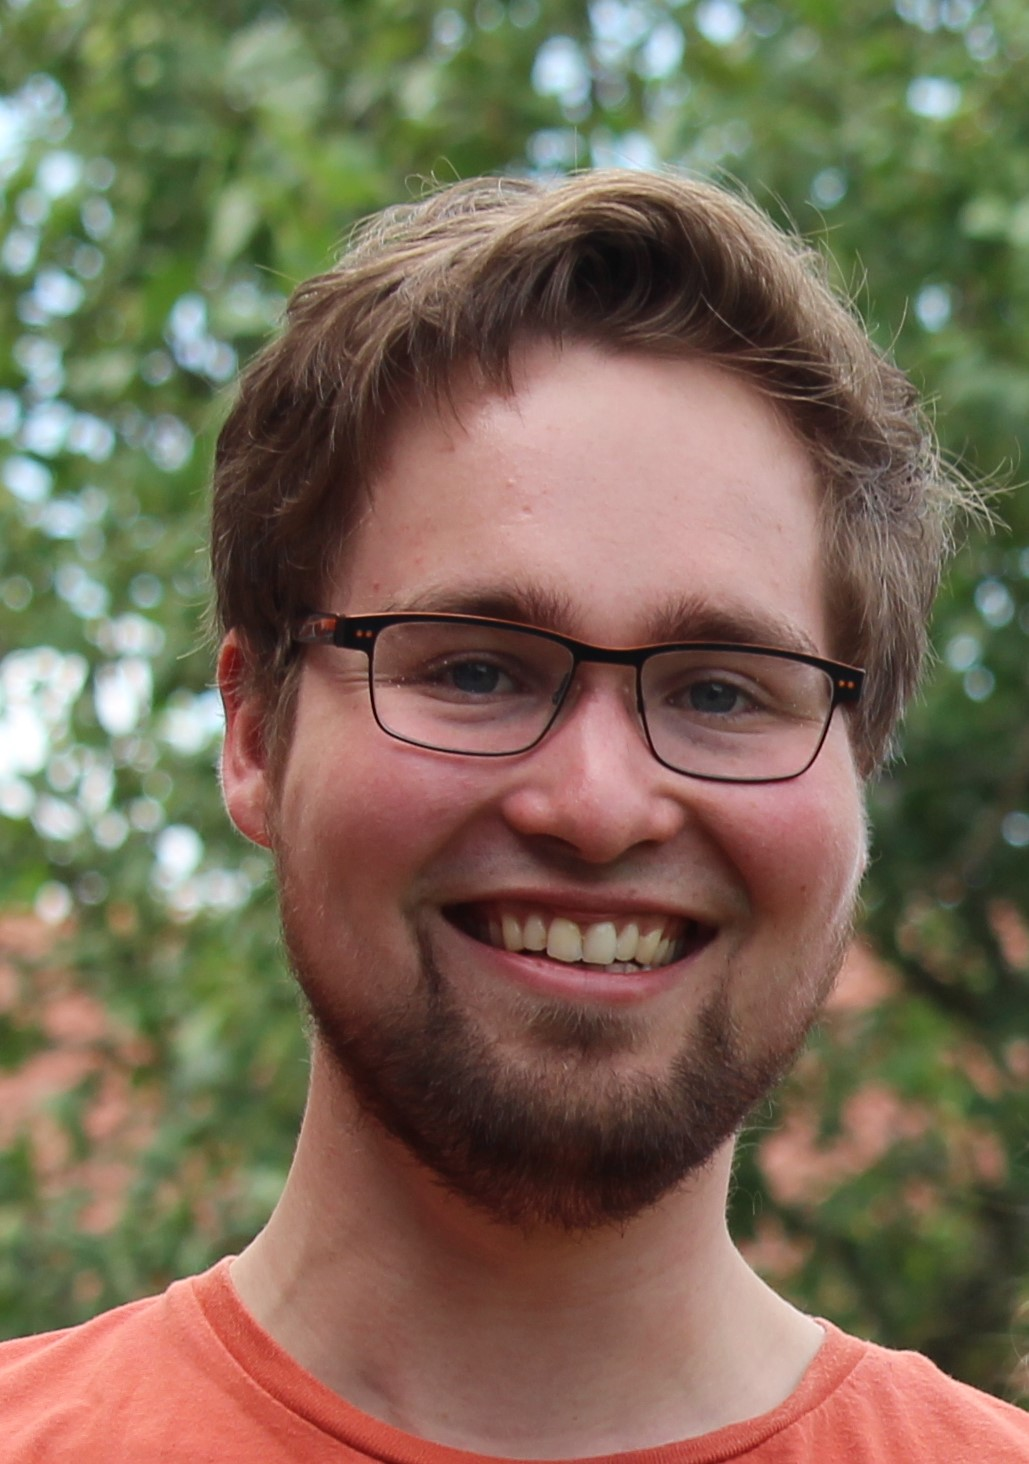
\includegraphics[width=\fibelstdlen]{res/vorstellungsfotos/Fotos Selbstvorstellungstexte Fibel/Jonas L.jpg}
	\end{wrapfigure}
}
{
Moin zusammen! Ich bin Jonas und studiere mittlerweile im Master Physik. In meinem Bachelor habe ich außerdem ziemlich viel Mathe gemacht (und bin da auch eigentlich immer noch nicht ganz von losgekommen). 
Zudem bin ich im Moment Vorsitzender der Fachschaft. Wenn ihr also Fragen zum Nebenfach Mathe oder zur Fachschaft an sich habt, bin ich ein guter Ansprechpartner. :-)
}

\vspace{-0.6cm}

\fibelvorstellung{
	\begin{wrapfigure}{r}{0cm}
		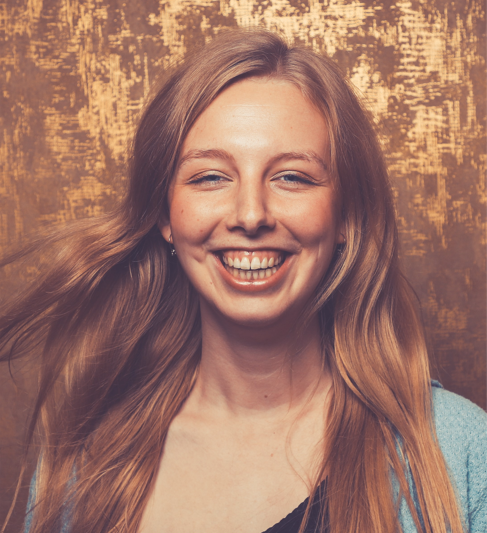
\includegraphics[width=\fibelstdlen]{res/vorstellungsfotos/Anna N_cut.PNG}
	\end{wrapfigure}
}
{
Hej, ich heiße Anna und bin gerade mit meiner Masterarbeit beschäftigt. 
Bei Fragen rund ums Studium und Münster könnt ihr mich gerne ansprechen. 
Ansonsten wünsche ich euch an dieser Stelle einen wunderschönen Start ins Studium.:)
}

\fibelvorstellung{
	\begin{wrapfigure}{l}{0cm}
		\includegraphics[width=\fibelstdlen]{res/vorstellungsfotos/benedikt_bieringer.png}
	\end{wrapfigure}
}
{
Hallo zusammen! Mein Name ist Benedikt. In der Fachschaft beschäftige ich mich unter anderem mit Computergrafik/Design. 
Programmieren und Schwimmen sind nur zwei meiner weiteren Freizeitbeschäftigungen. 
In meinen mittlerweile schon 14~Semestern Fachschafts- und Studienerfahrung kann ich euch aber auch bei einer ganzen Reihe weiterer Fragen weiterhelfen.
}

\vspace{-0.6cm}

\fibelvorstellung{
	\begin{wrapfigure}{r}{0cm}
		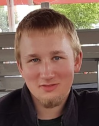
\includegraphics[width=\fibelstdlen]{res/vorstellungsfotos/hauke_hawighorst.jpg}
	\end{wrapfigure}
}
{
Moin, ich heiße Hauke und bin seit 2016 an der Uni und in der Fachschaft. Als Erasmus Student war ich in Sevilla (Spanien) und in Münster bin ich für die Evaluation der Lehre zuständig. 
Euch ein herzliches Willkommen in Münster!
}

\fibelvorstellung{
	\begin{wrapfigure}{l}{0cm}
		\includegraphics[width=\fibelstdlen]{res/vorstellungsfotos/jan_honermann.jpg}
	\end{wrapfigure}
}
{
Hi, ich bin Jan und sitze gerade an meiner Doktorarbeit. Falls ihr Fragen habt, könnt ihr euch gerne an mich wenden, ich bin meistens netter, als ich aussehe. ;)
}

\vspace{0.1cm}

\fibelvorstellung{
	\begin{wrapfigure}{r}{0cm}
		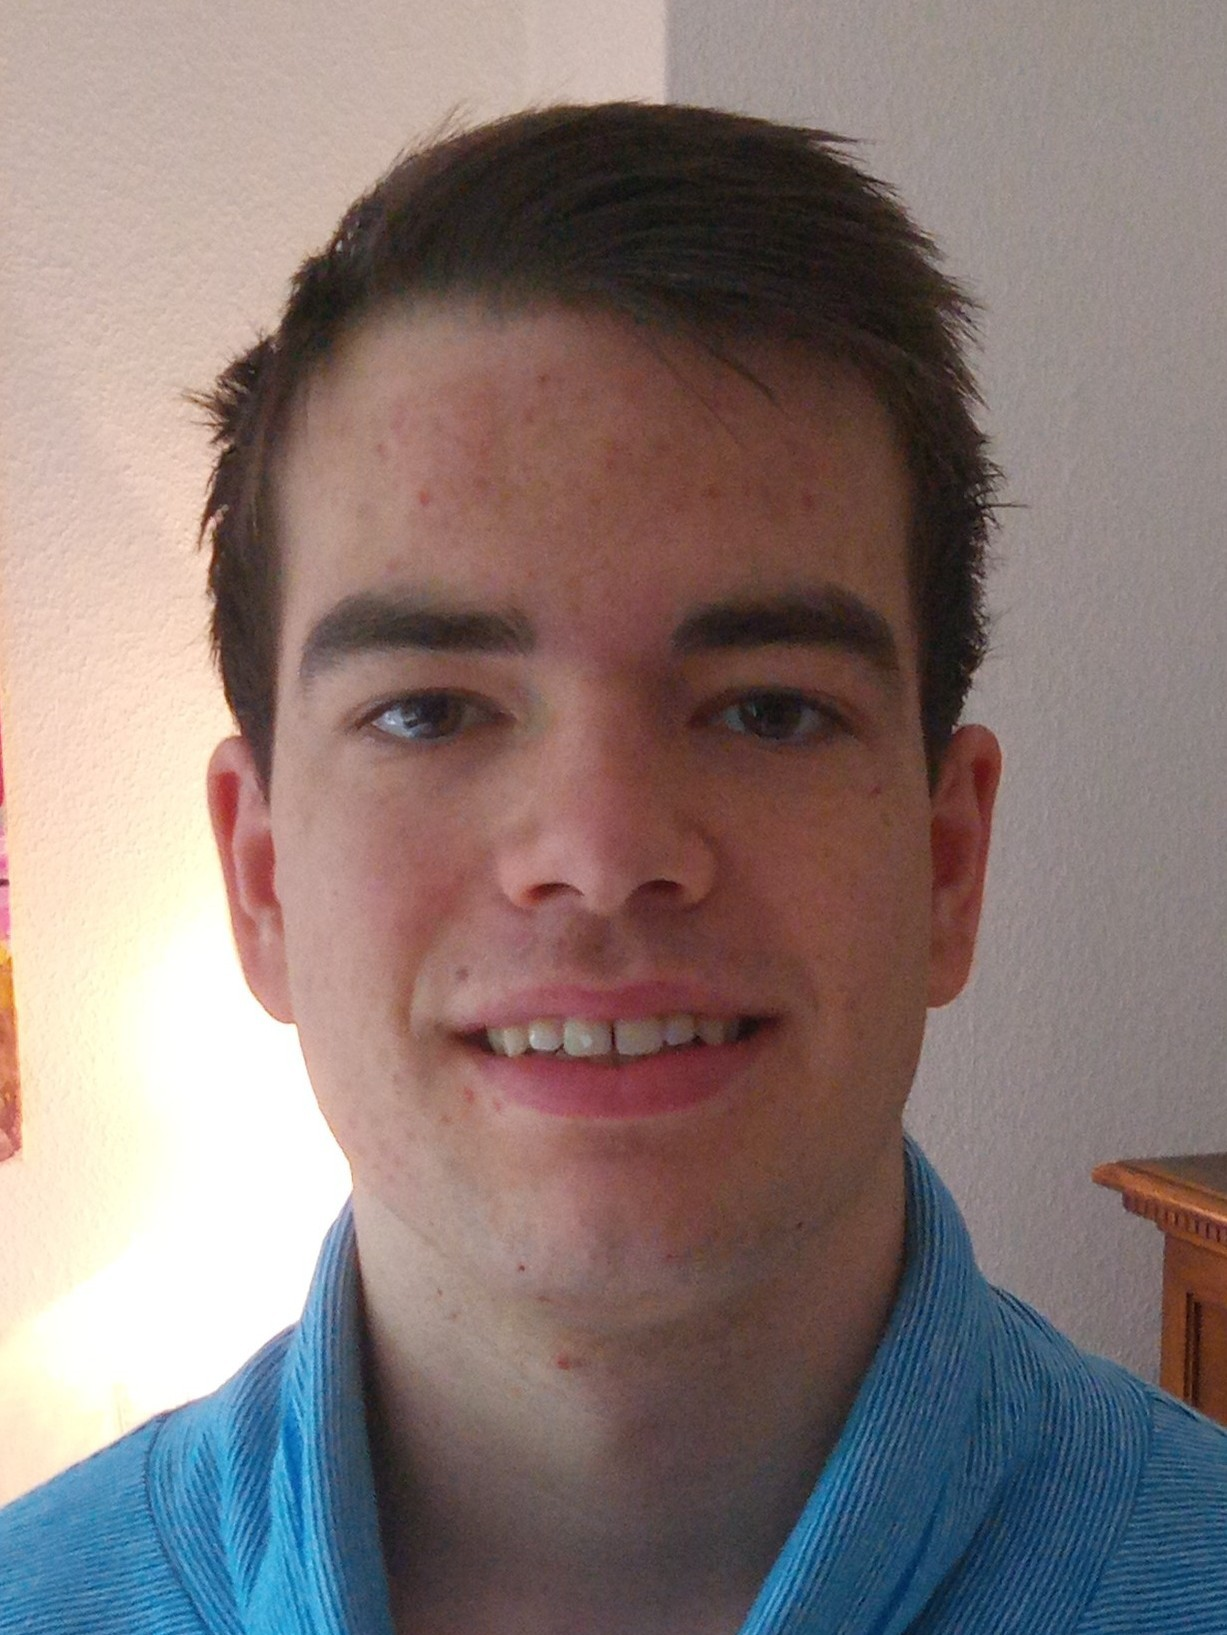
\includegraphics[width=\fibelstdlen]{res/vorstellungsfotos/Fotos Selbstvorstellungstexte Fibel/Lambert.jpg}
	\end{wrapfigure}
}
{
Hallo, ich bin Lambert und jetzt im 3. Semester meines Physikbachelors. Ich vertrete die Fachschaft auf der Fachschaftenkonferenz und helfe ein wenig bei der Evaluation mit. 
Ihr könnt mir gerne alle möglichen Fragen zum Studium und auch anderen Themen stellen. Es ist aber gut möglich, dass ich die Antwort nicht kenne. 
Willkommen in Münster und einen schönen Studiumsbeginn!
}

\vspace{-0.5cm}

\fibelvorstellung{
	\begin{wrapfigure}{l}{0cm}
		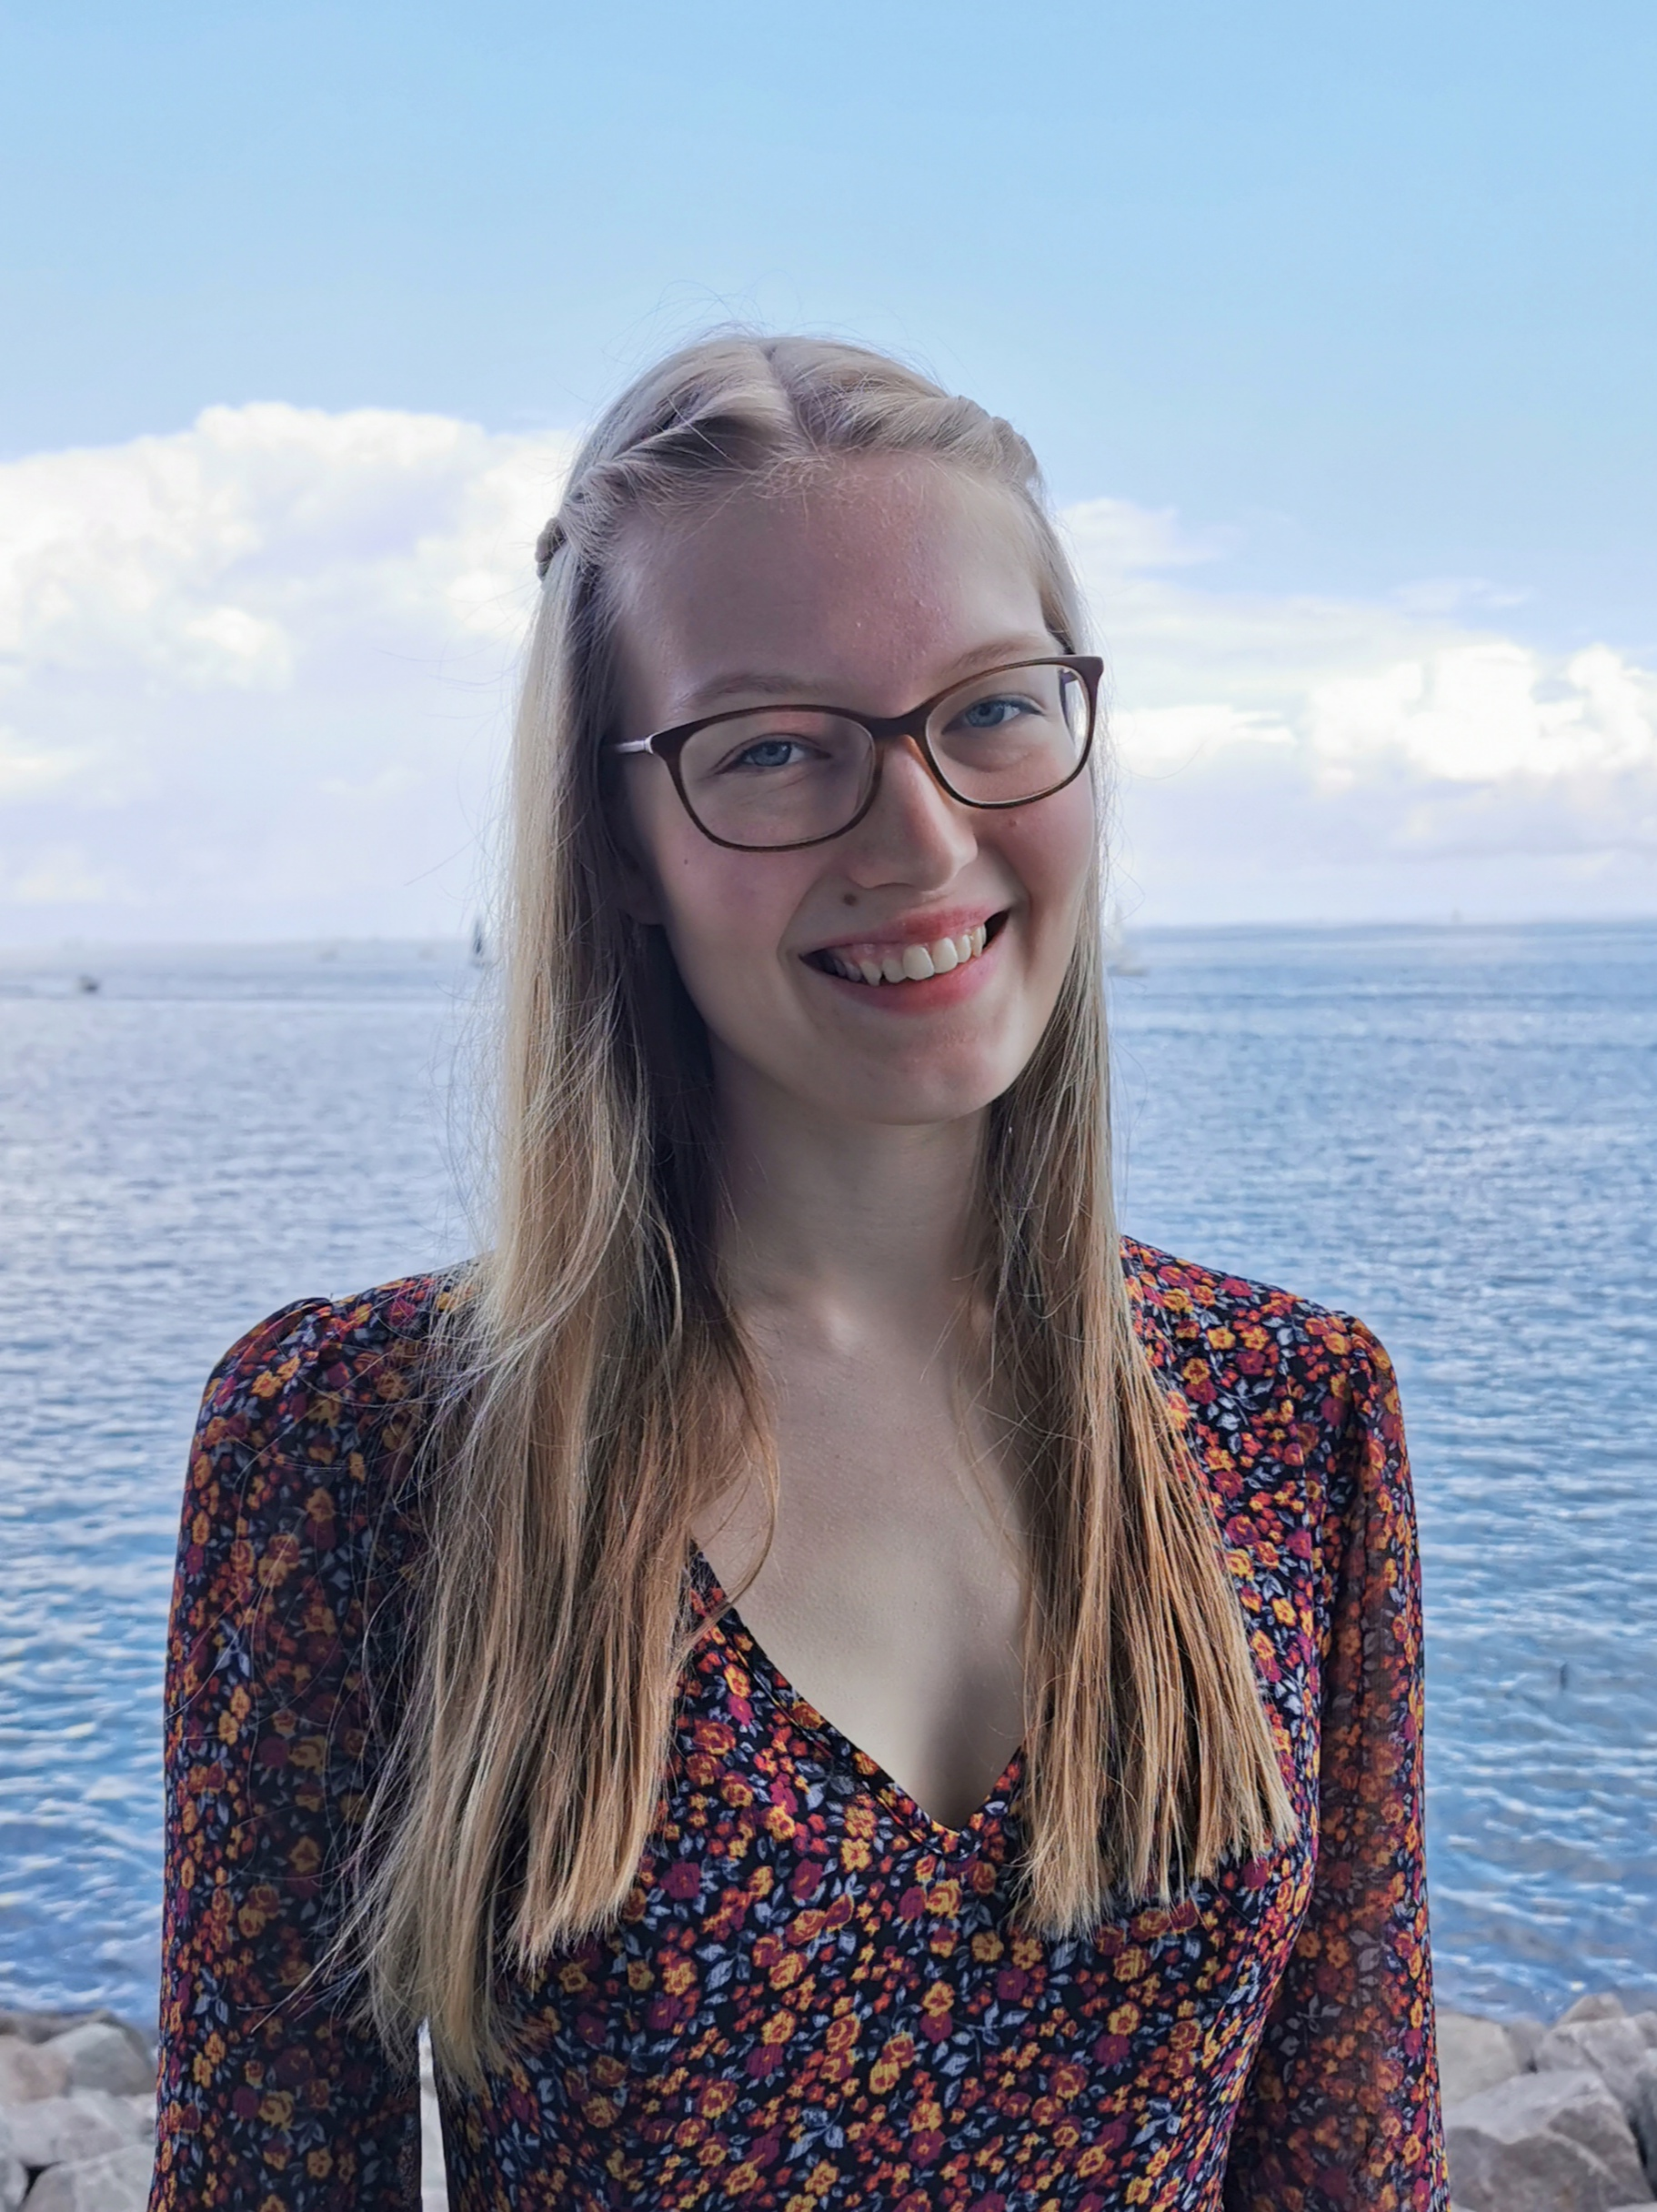
\includegraphics[width=\fibelstdlen]{res/vorstellungsfotos/paula_mors.jpg}
	\end{wrapfigure}
}
{
Huhu, ich bin Paula und seit dem Sommersemester 2019 in der Fachschaft. Neben Fragen Rund um das Studium könnt ihr mich auch gerne auf royale Hochzeiten oder Filme mit Audrey Hepburn ansprechen. 
Ich wünsche euch einen lustigen Start ins Physikstudium!
}

\fibelvorstellung{
	\begin{wrapfigure}{r}{0cm}
		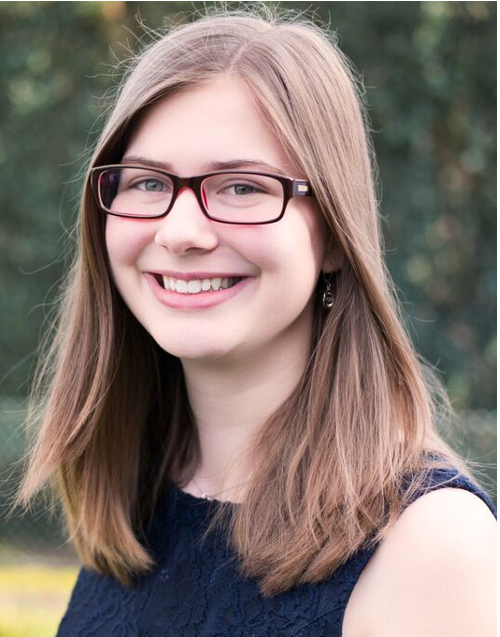
\includegraphics[width=\fibelstdlen]{res/vorstellungsfotos/Sandra_cut.PNG}
	\end{wrapfigure}
}
{
Hi :), mein Name ist Sandra, bin 20 und ich studiere inzwischen im 5. Semester Physik. Bei Fragen könnt ihr euch gerne an mich wenden. 
Ansonsten wünsche ich euch erst einmal viel Spaß in der O-Woche! 
}

\fibelvorstellung{
	\begin{wrapfigure}{l}{0cm}
		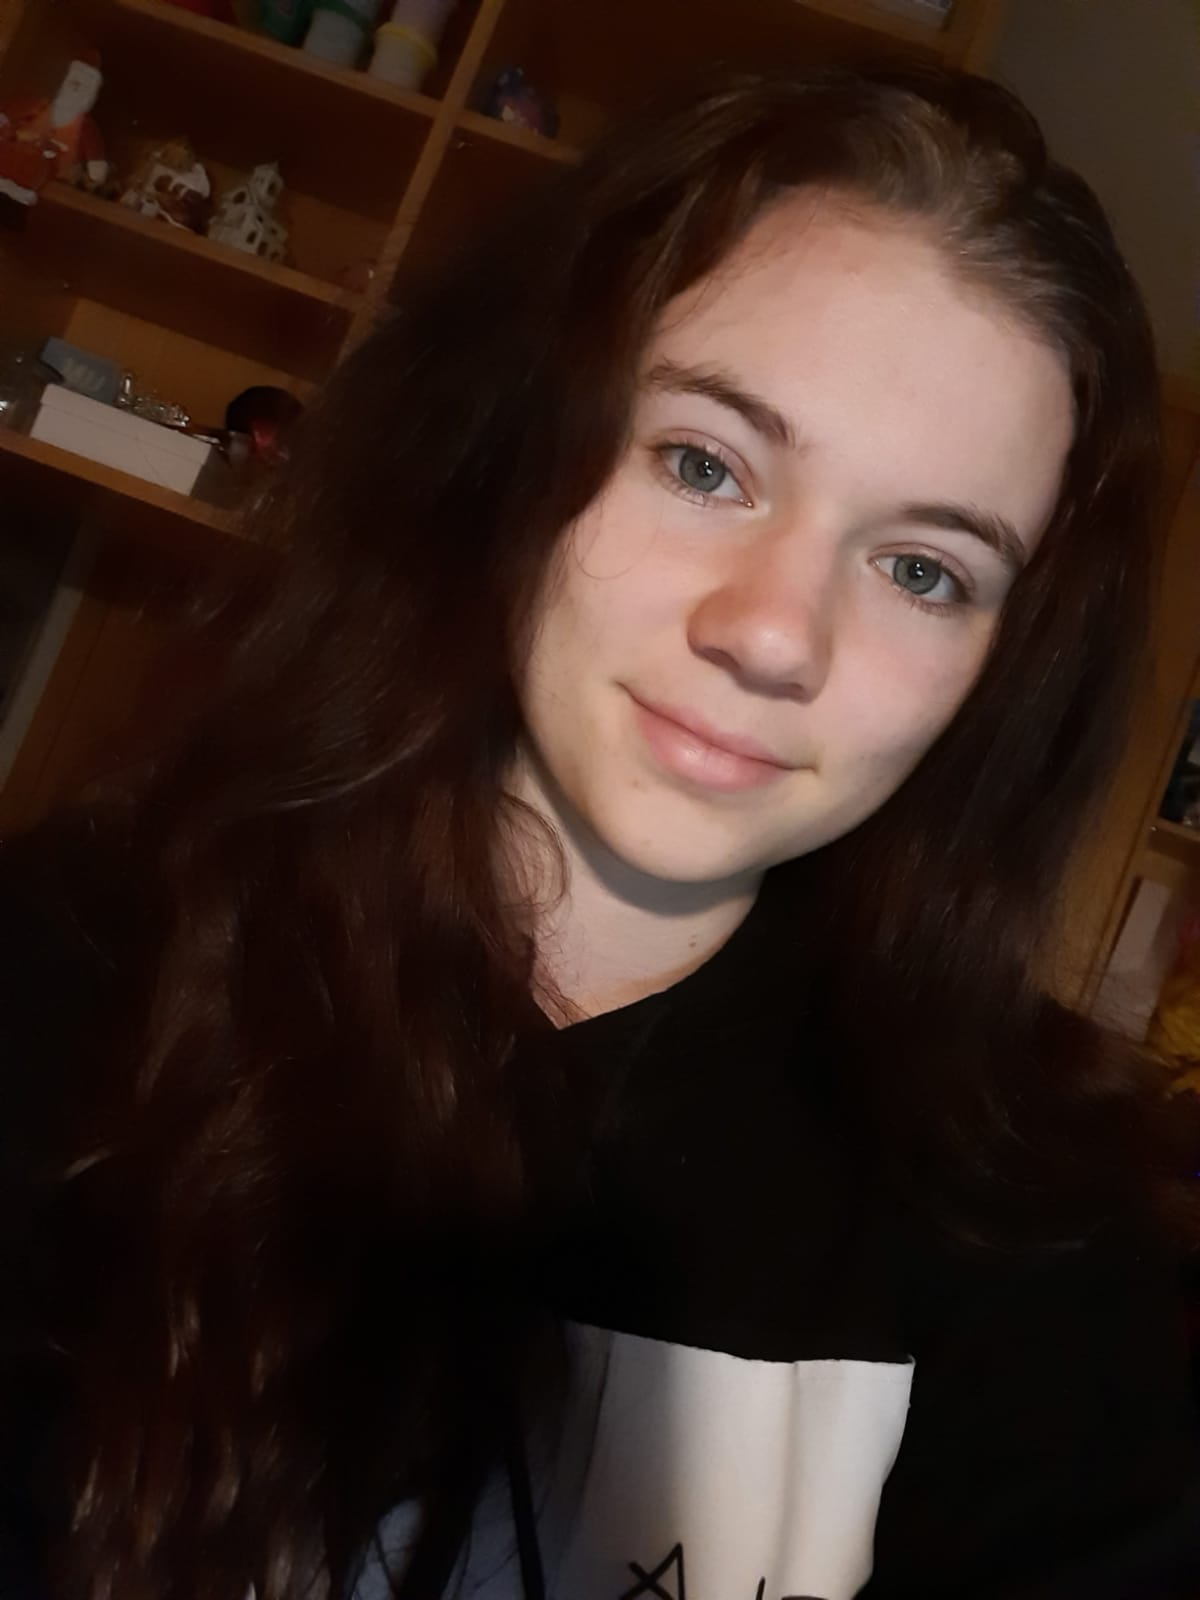
\includegraphics[width=\fibelstdlen]{res/vorstellungsfotos/Fotos Selbstvorstellungstexte Fibel/Anna T.JPEG}
	\end{wrapfigure}
}
{
Heyo, ich bin Anna und studiere ab jetzt im fünften Semester Physik. 
Ich hoffe ihr habt alle viel Spaß in der O-Woche und schafft es gut ins Studium, hoffentlich diesmal tatsächlich in Präsenz.:)
}

\fibelvorstellung{
	\begin{wrapfigure}{r}{0cm}
		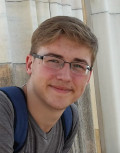
\includegraphics[width=\fibelstdlen]{res/vorstellungsfotos/christoph_wesseler.jpeg}
	\end{wrapfigure}
}
{
Sehr geehrte Erstis: Moin!
Ich bin Christoph und studiere im 3. Semester Physik. In der Fachschaft bin ich im O-Wochen Team und beim Sommerfest tätig. Wenn Ihr Fragen habt, z.B zur O-Woche oder zum etwas Chaotischen Alltag an der Uni, immer her damit, es lebe das Chaos! :D 
Ich wünsche euch allen eine schöne O-Woche und hoffe man sieht sich mal in der Fachschaft.
}

% \vspace{-0.8cm}

\fibelvorstellung{
	\begin{wrapfigure}{l}{0cm}
		\includegraphics[width=\fibelstdlen]{res/vorstellungsfotos/marius_willer_cropped.jpg}
	\end{wrapfigure}
}
{
Hi, ich bin Marius und heiße euch ebenfalls herzlich willkommen hier in Münster. Wenn ihr die Stadt noch nicht richtig kennt, dann freut euch darauf, sie kennenzulernen. 
Das Studium wird zwar zwischendurch etwas schwierig, aber lasst euch trotzdem nicht die Freude dran nehmen. ¡Mucha suerte!\footnote{\url{https://www.youtube.com/watch?v=iik25wqIuFo}}
}

\fibelvorstellung{
	\begin{wrapfigure}{r}{0cm}
		\includegraphics[width=\fibelstdlen]{res/vorstellungsfotos/lukas_eschmann_cropped.jpg}
	\end{wrapfigure}
}
{
Moin liebe Erstis, mein Name ist Lukas und schon seit 2012 in der Fachschaft. Mein "normales" Studium habe ich bereits abgeschlossen, kann also so ziemlich alle Fragen zum Studium beantworten.
Ich bin mittlerweile im Promotionsstudiengang angekommen und bin nur noch wenig in Hörsälen oder dem Fachschaftsraum anzutreffen.
Auch Fragen zu Forschungsschwerpunkten der Uni oder aktuellen Themen der Forschung könnt ihr mir gerne stellen.
}

\vspace{-0.8cm}

\fibelvorstellung{
	\begin{wrapfigure}{l}{0cm}
		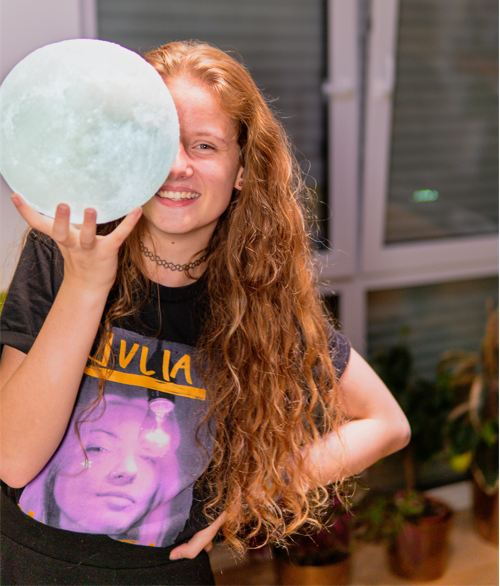
\includegraphics[width=\fibelstdlen]{res/vorstellungsfotos/Eva_cut.PNG}
	\end{wrapfigure}
}
{
Hey, ich heiße Eva und studiere im 5. Semester Physik. Seit dem Sommersemester 2020 bin ich in der Fachschaft und nun stellvertretende Vorsitzende. Außerdem betätigte ich mich im Design-Team und in der Öffentlichkeitsarbeit. 
Ich wünsche Euch einen tollen Start ins Studium! PS: Über ein freundliches "Hallo" (auf dem Gang, im Vorbeigehen) freue ich mich immer.
} 

\vspace{-1.8cm}

\fibelvorstellung{
	\begin{wrapfigure}{r}{0cm}
		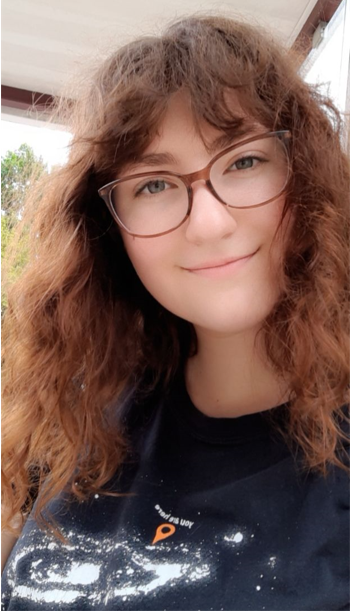
\includegraphics[width=\fibelstdlen]{res/vorstellungsfotos/Hannah_cut.PNG}
	\end{wrapfigure}
}
{
Hallihallo ich bin Hannah, ich studiere seit dem WS 19/20 Physik und bin auch schon genauso lange in der Fachschaft. 
Bei dieser bin verantwortlich für das Sommerfest und die Erstisphibel. Ich wünsche euch einen entspannten Start ins Semester! :)
}

\vspace{0.2cm}

\fibelvorstellung{
	\begin{wrapfigure}{l}{0cm}
		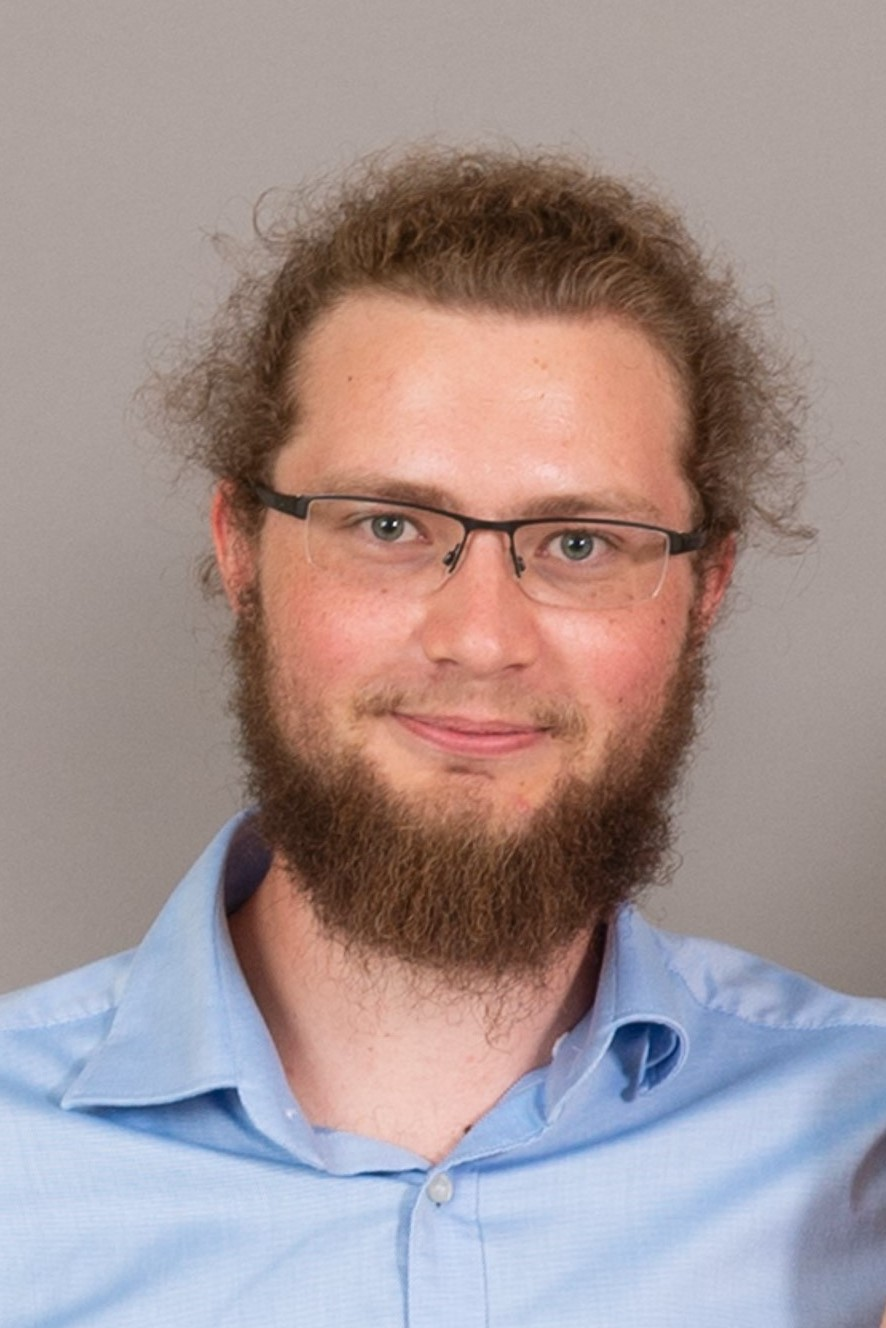
\includegraphics[width=\fibelstdlen]{res/vorstellungsfotos/Fotos Selbstvorstellungstexte Fibel/Ali Neuwirth.jpg}
	\end{wrapfigure}
}
{
Hallo Welt! Ich verkehre unter den Namen Alexander, Alekschander, Alex, Xander, Ali, Puck und Pucky. Bald geht es bei mir mit der Promotion los. 
In der Fachschaft beschäftige ich mich mit IT-Administration. Entsprechend kann ich bei Fragen zu Physik und Technik gerne helfen. \texttt{\kern-0.25ex\raisebox{0.25ex}{\rotatebox{45}{\raisebox{-.75ex}\grqq\kern-1.5ex\rotatebox{-90})}}\kern-0.5ex}
}

\fibelvorstellung{
	\begin{wrapfigure}{r}{0cm}
		
\includegraphics[width=\fibelstdlen]{res/vorstellungsfotos/Fotos Selbstvorstellungstexte Fibel/Bild_Moritz.jpg}
	\end{wrapfigure}
}
{
Moin, ich bin Moritz und jetzt seit 3 Semestern in der Fachschaft. Ich studiere im Zwei-Fach-Bachelor Physik und Chemie, bei Fragen zum Lehramtsstudium dürft ihr mich also gerne ansprechen. 
Ich wünsche euch einen erfolgreichen Start ins Studium und insbesondere für die ZFB möglichst wenig Überschneidungen in euren Stundenplänen. :)
}

\fibelvorstellung{
	\begin{wrapfigure}{l}{0cm}
		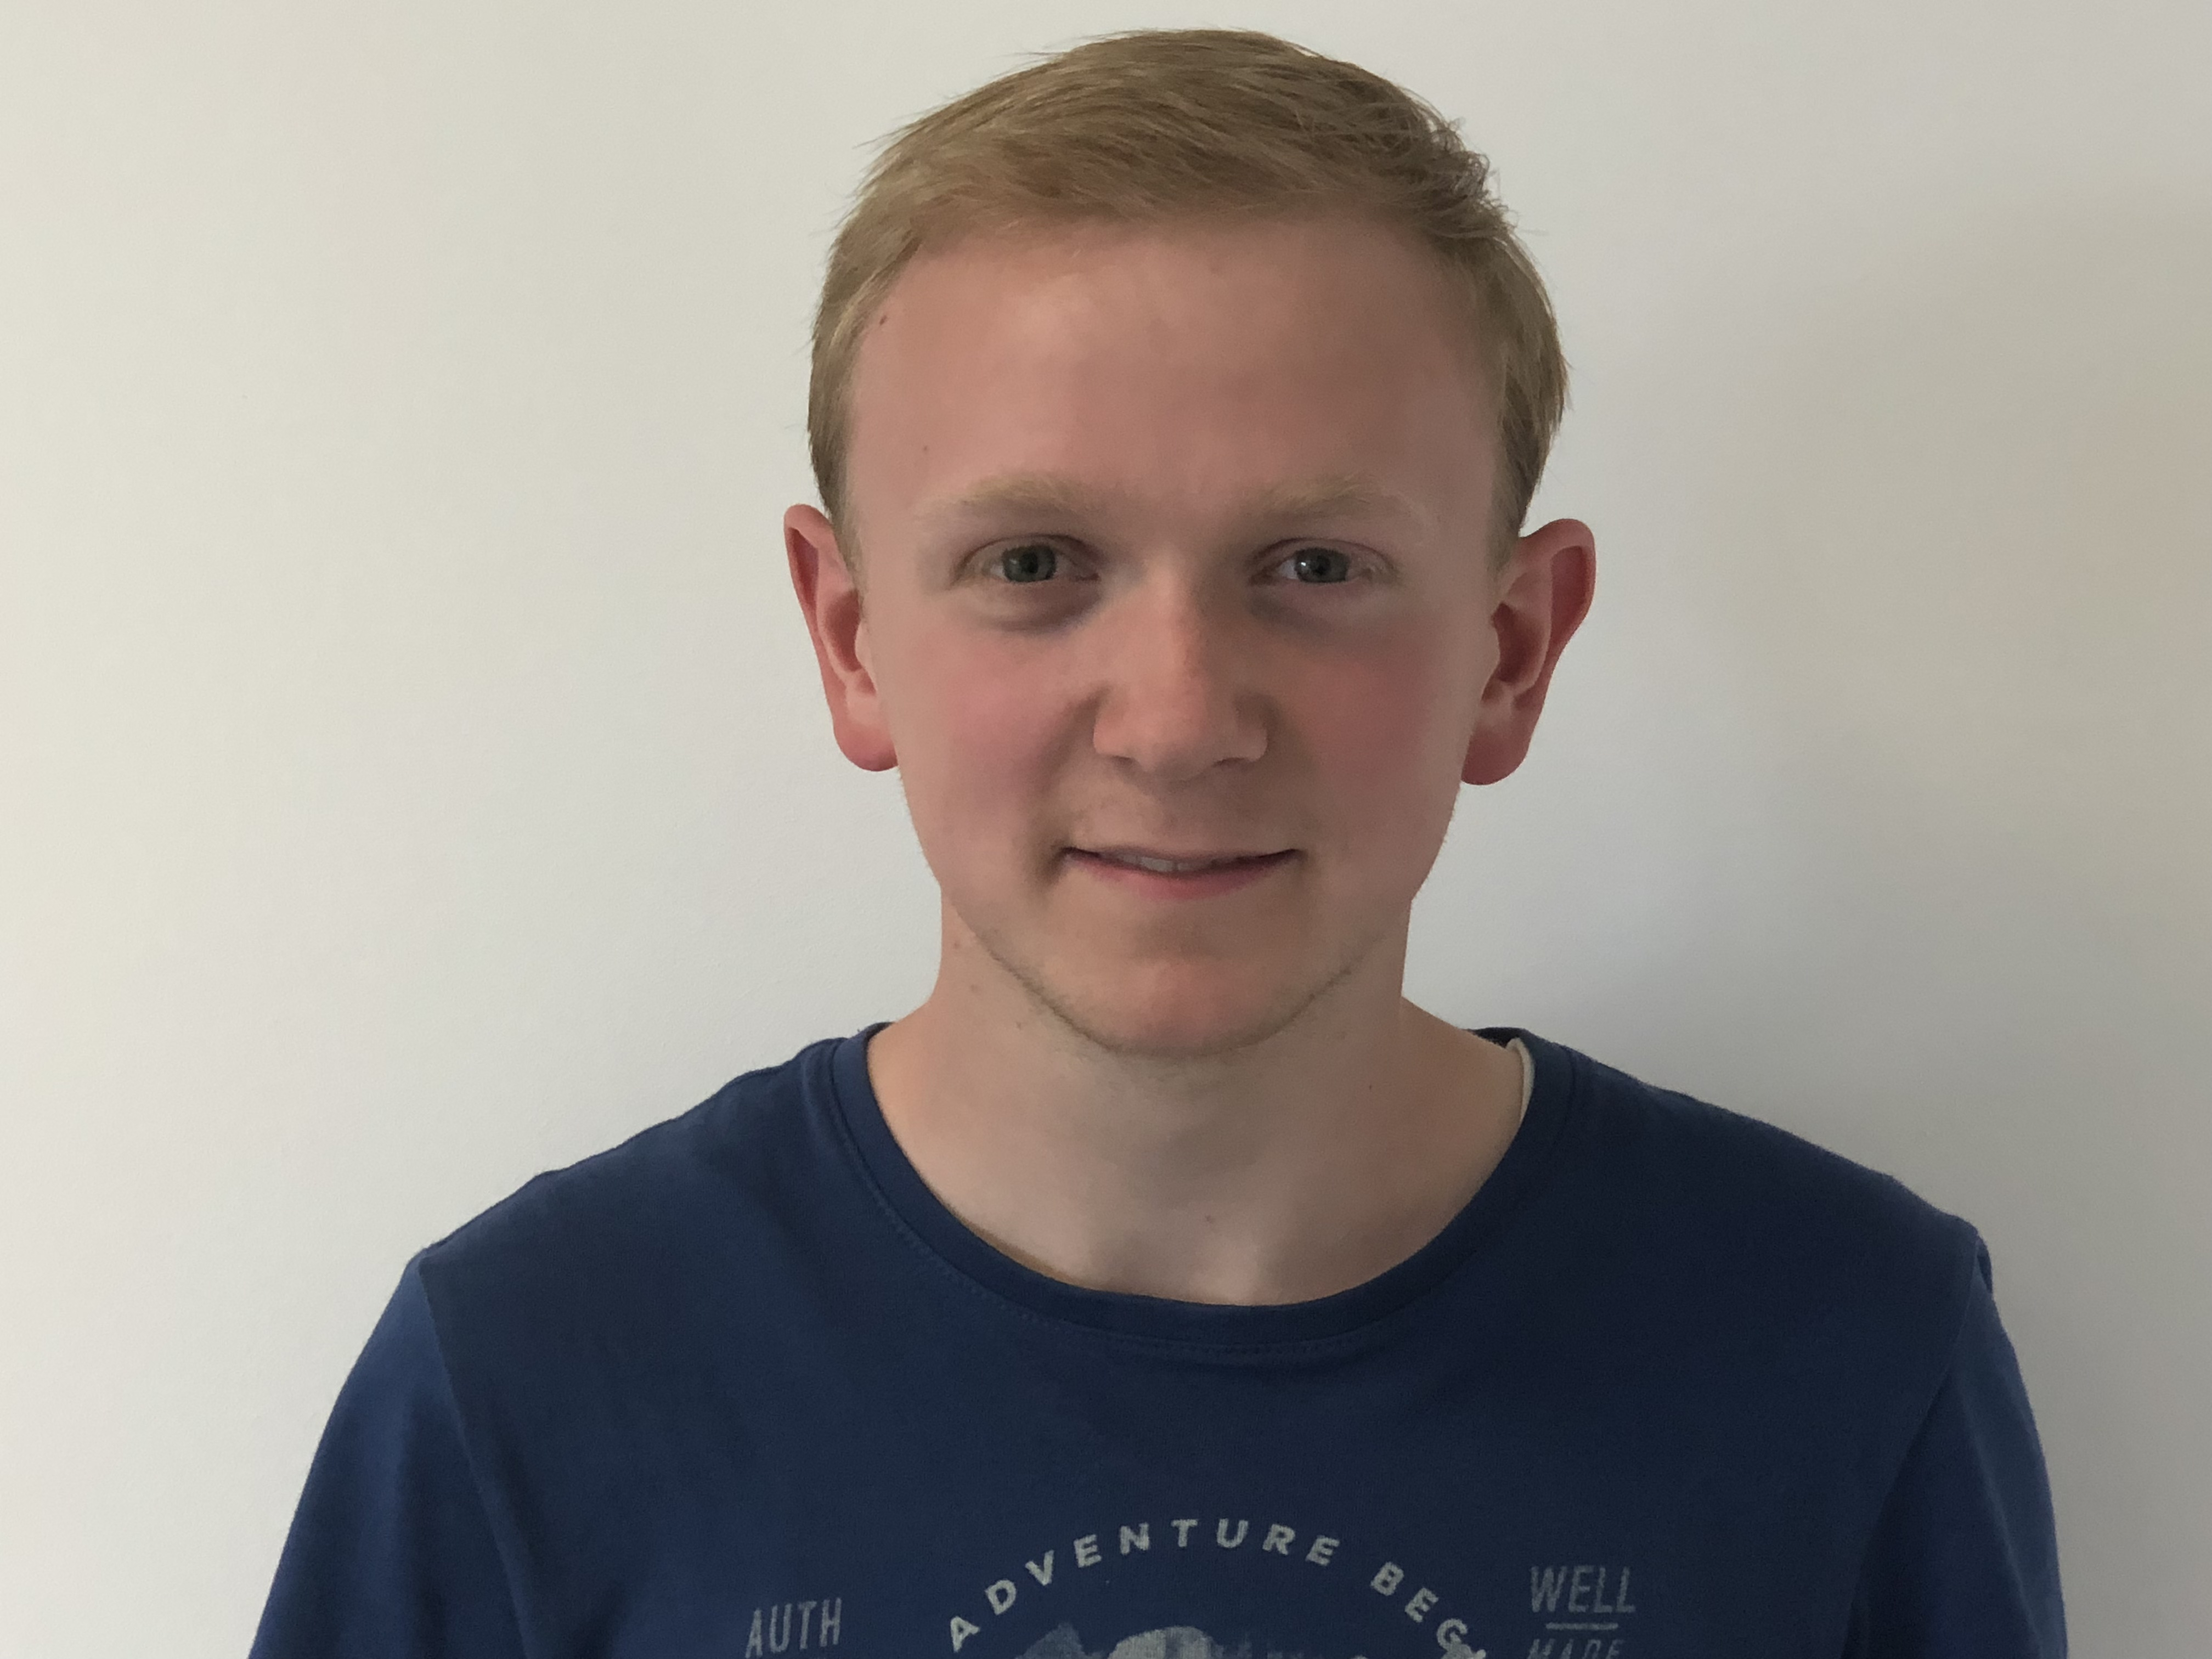
\includegraphics[width=\fibelstdlen]{res/vorstellungsfotos/Fotos Selbstvorstellungstexte Fibel/tim_stellhorn.jpg}
	\end{wrapfigure}
}
{
Hej Leute, ich bin Tim und studiere Physik im Master. Ich kann euch nur sagen, lasst euch auf keinen Fall von einem vielleicht etwas schwierigen Einstieg verunsichern, das war für keinen von uns leicht. 
Erstmal aber möchte ich euch noch viel Spaß in der O-Woche wünschen und hoffe, dass ihr die Möglichkeit bekommt, einige andere Erstis kennen zu lernen. 
Bei Fragen kommt gerne zu mir; besonders beim Erasmusprogramm kann ich euch weiterhelfen, denn ich war selber im letzten Jahr in Lund. Also, habt eine schöne Zeit und vielleicht läuft man sich ja mal in der Uni über den Weg. ;-)
}



%
% \begin{center}
% 	\includegraphics[width=\columnwidth]{res/fsphys_logo.pdf}
% \end{center}
%
%
%

\vspace{6ex}

\fibelvorstellung{
	\begin{wrapfigure}{r}{0cm}
		\includegraphics[width=\fibelstdlen]{res/vorstellungsfotos/fritz.png}
	\end{wrapfigure}
}
{
Hallo, ich bin Fritz und bin schon  in der Fachschaft Physik.
Die Mannschaft hier ist echt genial aufgestellt. Dadurch macht es richtigen Spaß, ein aktiver Teil der Universität Münster zu sein.
Ich kann dir nur empfehlen: Mach' mit und verändere die Uni!
}


\end{multicols}

\vspace{20ex}
